\documentclass[tikz,border=8pt]{standalone}
\usepackage[utf8]{inputenc}\usetikzlibrary{positioning,fit,arrows.meta,shapes.geometric}
\definecolor{navy}{HTML}{17365D}\definecolor{gold}{HTML}{C69214}\definecolor{soft}{HTML}{FFF7DD}
\tikzset{actor/.style={draw=navy,rounded corners,fill=white,minimum width=3.1cm,minimum height=.75cm,font=\bfseries\small},usecase/.style={draw=gold,ellipse,fill=soft,minimum width=6.4cm,minimum height=.82cm,align=center,font=\small},link/.style={draw=navy,-{Latex[length=2mm]},thin}}
\begin{document}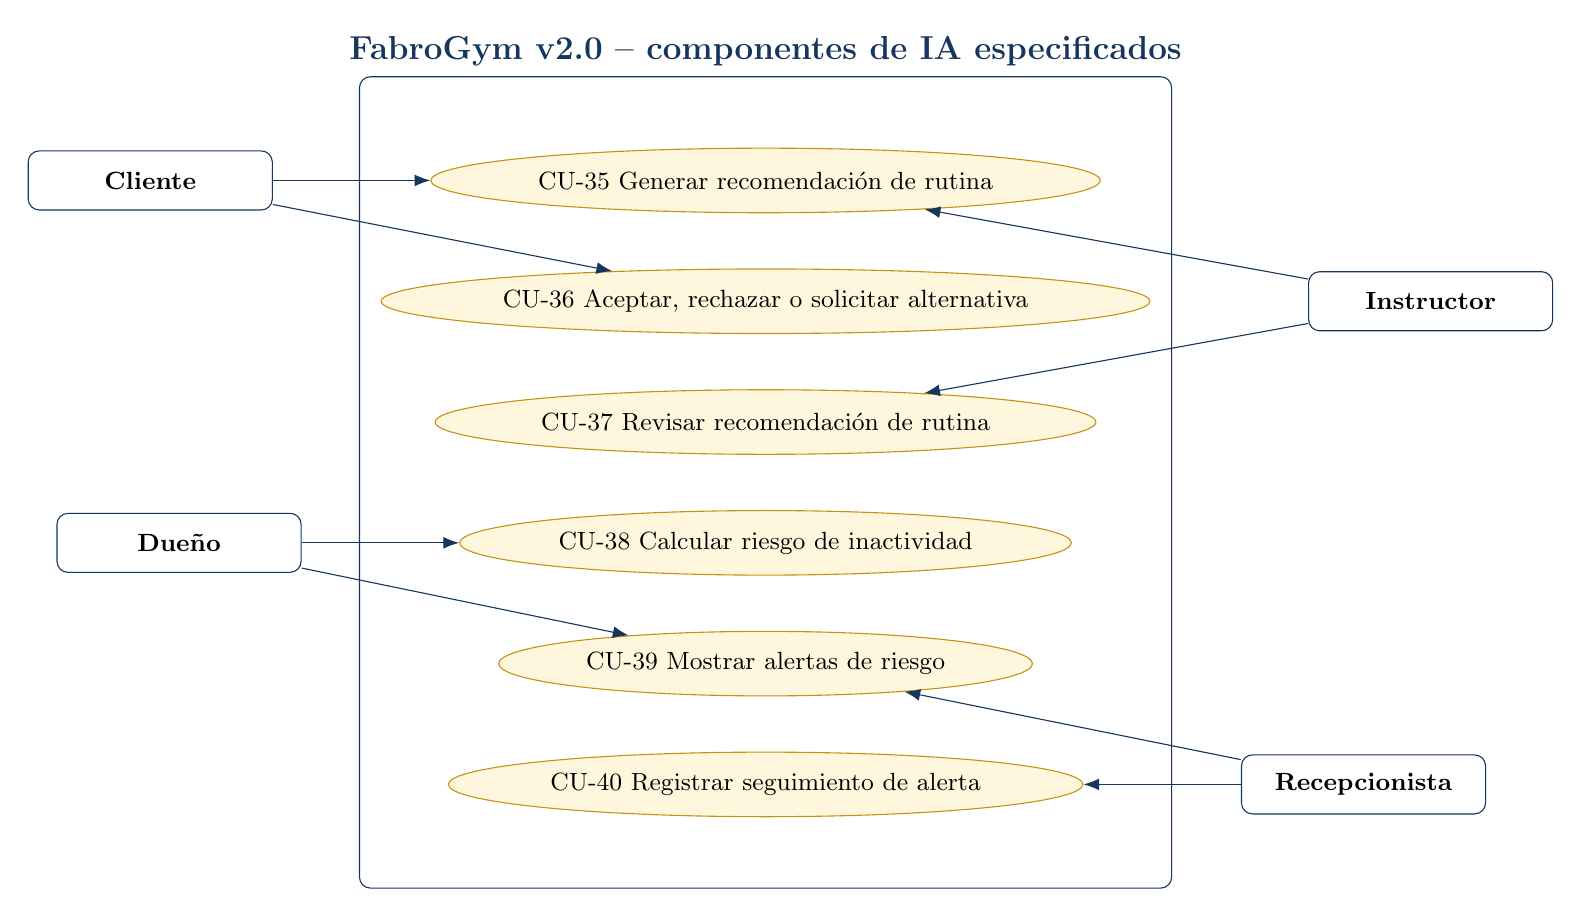
\begin{tikzpicture}[node distance=7mm and 18mm]
\node[usecase] (c35) {CU-35 Generar recomendación de rutina};
\node[usecase,below=of c35] (c36) {CU-36 Aceptar, rechazar o solicitar alternativa};
\node[usecase,below=of c36] (c37) {CU-37 Revisar recomendación de rutina};
\node[usecase,below=of c37] (c38) {CU-38 Calcular riesgo de inactividad};
\node[usecase,below=of c38] (c39) {CU-39 Mostrar alertas de riesgo};
\node[usecase,below=of c39] (c40) {CU-40 Registrar seguimiento de alerta};
\node[draw=navy,rounded corners,fit=(c35)(c40),inner sep=9mm,label={[font=\bfseries\large,text=navy]above:FabroGym v2.0 -- componentes de IA especificados}] {};
\node[actor,left=20mm of c35] (cl) {Cliente};
\node[actor,right=20mm of c36] (ins) {Instructor};
\node[actor,left=20mm of c38] (du) {Dueño};
\node[actor,right=20mm of c40] (re) {Recepcionista};
\foreach \x in {c35,c36}\draw[link] (cl)--(\x);
\foreach \x in {c35,c37}\draw[link] (ins)--(\x);
\foreach \x in {c38,c39}\draw[link] (du)--(\x);
\foreach \x in {c39,c40}\draw[link] (re)--(\x);
\end{tikzpicture}\end{document}
